\documentclass[letterpaper]{article}
\usepackage[margin=1in]{geometry}
\usepackage[utf8]{inputenc}
\usepackage{textcomp}
\usepackage{amssymb}
\usepackage{natbib}
\usepackage{graphicx}
\usepackage{gensymb}
\usepackage{amsthm, amsmath, mathtools}
\usepackage[dvipsnames]{xcolor}
\usepackage{enumerate}
\usepackage{mdframed}
\usepackage[most]{tcolorbox}
\usepackage{csquotes}
% https://tex.stackexchange.com/questions/13506/how-to-continue-the-framed-text-box-on-multiple-pages

\tcbuselibrary{theorems}

\newcommand{\R}{\mathbb{R}}
\newcommand{\Z}{\mathbb{Z}}
\newcommand{\N}{\mathbb{N}}
\newcommand{\Q}{\mathbb{Q}}
\newcommand{\C}{\mathbb{C}}
\newcommand{\code}[1]{\texttt{#1}}
\newcommand{\mdiamond}{$\diamondsuit$}
\newcommand{\PowerSet}{\mathcal{P}}
\newcommand{\Mod}[1]{\ (\mathrm{mod}\ #1)}
\DeclareMathOperator{\lcm}{lcm}

%\newtheorem*{theorem}{Theorem}
%\newtheorem*{definition}{Definition}
%\newtheorem*{corollary}{Corollary}
%\newtheorem*{lemma}{Lemma}
\newtheorem*{proposition}{Proposition}


\newtcbtheorem[number within=section]{theorem}{Theorem}
{colback=green!5,colframe=green!35!black,fonttitle=\bfseries}{th}

\newtcbtheorem[number within=section]{definition}{Definition}
{colback=blue!5,colframe=blue!35!black,fonttitle=\bfseries}{def}

\newtcbtheorem[number within=section]{corollary}{Corollary}
{colback=yellow!5,colframe=yellow!35!black,fonttitle=\bfseries}{cor}

\newtcbtheorem[number within=section]{lemma}{Lemma}
{colback=red!5,colframe=red!35!black,fonttitle=\bfseries}{lem}

\newtcbtheorem[number within=section]{example}{Example}
{colback=white!5,colframe=white!35!black,fonttitle=\bfseries}{def}

\newtcbtheorem[number within=section]{note}{Important Note}{
        enhanced,
        sharp corners,
        attach boxed title to top left={
            xshift=-1mm,
            yshift=-5mm,
            yshifttext=-1mm
        },
        top=1.5em,
        colback=white,
        colframe=black,
        fonttitle=\bfseries,
        boxed title style={
            sharp corners,
            size=small,
            colback=red!75!black,
            colframe=red!75!black,
        } 
    }{impnote}
\usepackage[utf8]{inputenc}
\usepackage[english]{babel}
\usepackage{fancyhdr}
\usepackage[hidelinks]{hyperref}

\pagestyle{fancy}
\fancyhf{}
\rhead{MATH 155A}
\chead{Thursday, April 07, 2022}
\lhead{Lecture 4}
\rfoot{\thepage}

\setlength{\parindent}{0pt}

\begin{document}

% 2.5: https://www.youtube.com/watch?v=IplJmjmneSo

\section{Graphics Pipeline, Linear \& Affine Transformations in \texorpdfstring{$\R^2$}{R2}}

\subsection{Inverses of Linear and Affine Transformations}
We begin with a definition. 
\begin{definition}{}{}
    Let $A$ and $B$ be transformations of $\R^2$. We say that $B$ is the \textbf{inverse} of $A$, written $B = A^{-1}$, if: 
    \begin{enumerate}
        \item $A \circ B = I$. 
        \item $B \circ A = I$. 
    \end{enumerate}
\end{definition}

\subsubsection{Finding Inverses of Linear Transformations}
How do we compute inverses? One way to do so is to do it by matrices. Let $A: \R^2 \mapsto \R^2$ be represented by the matrix $M = \begin{bmatrix}
    a & b \\ c & d
\end{bmatrix}$. Then, $A^{-1}$ is represented by $M^{-1}$, where 
\[M^{-1} = \begin{bmatrix}
    d & -b \\ 
    -c & a
\end{bmatrix} \frac{1}{ad - bc}.\]

\subsubsection{Finding Inverses of Affine Transformations}
Let $A(\mathbf{x})$ be defined by 
\[A(\mathbf{x}) = B(\mathbf{x}) + \mathbf{u},\]
where $B$ is linear and $\mathbf{u} \in \R$ so that $A$ is affine. How do we compute its inverse? Now, to find $A^{-1}$, we need to solve 
\[\mathbf{y} = B(\mathbf{x}) + \mathbf{u}\]
to get $\mathbf{x}$ in terms of $\mathbf{y}$. Now, we have 
\begin{equation*}
    \begin{aligned}
        \mathbf{y} &= B(\mathbf{x}) + \mathbf{u} \\ 
            &\implies B(\mathbf{x}) = \mathbf{y} - \mathbf{u} \\ 
            &\implies \mathbf{x} = B^{-1}(\mathbf{y} - \mathbf{u}) \\ 
            &\implies \mathbf{x} = B^{-1}(\mathbf{y}) - B^{-1}(\mathbf{u}) \\ 
            &\implies \mathbf{x} = \underbrace{B^{-1}(\mathbf{y})}_{\text{Linear Part}} + \overbrace{(-B^{-1}(\mathbf{u}))}^{\text{Translation Part}}.
    \end{aligned}
\end{equation*}

\subsection{Compositions and Generalized Rotations}
Recall that we have
\begin{itemize}
    \item Rotations: $R_{\theta}$.
    \item Scalings: $S_{\cyclic{\alpha, \beta}}$.
    \item Reflections.
\end{itemize}
We now want to discuss generalized rotations. Recall again that $R_{\theta}$ is a rotation about the \textbf{origin} $\theta$. A \textbf{generalized rotation}, denoted $R_{\theta}^{\mathbf{u}}$, where $\mathbf{u} \in \R^2$ and $\theta \in \R$, is a rotation about some arbitrary point $\mathbf{u}$. In other words, we hold $\mathbf{u}$ fixed and then rotate about $\mathbf{u}$ counter-clockwise through angle $\theta$. Consider the following example: 
\begin{center}
    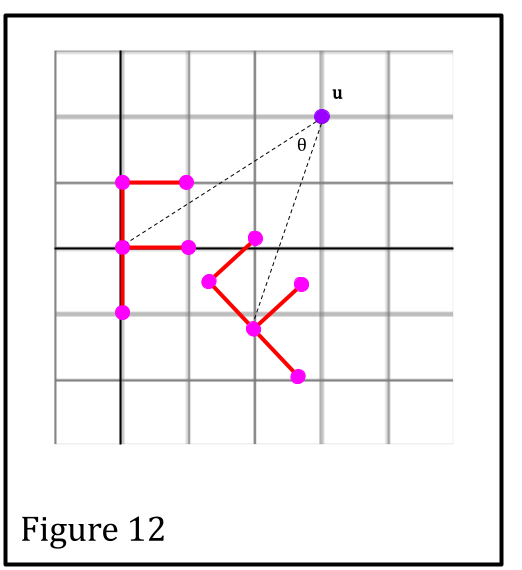
\includegraphics[scale=0.4]{../assets/f11.png}
\end{center}
In the figure above\footnote{Not drawn to scale.}, we have the \emph{image} of ``F'' under $R_{\theta}^{\mathbf{u}}$. Our goal is to be able to express $R_{\theta}^{\mathbf{u}}$ in terms of rotations (about the origin) and translations. For an example like the one above, we could:
\begin{enumerate}
    \item Move $\mathbf{u}$ to the origin $\mathbf{0}$; we call this $T_{-\mathbf{u}}$ (translation by $-\mathbf{u}$). 
    \item Perform the rotation about the origin $\mathbf{0}$; we call this $R_{\theta}$ (counter-clockwise rotation about the origin $\theta$ degrees).
    \item Then, move $\mathbf{0}$ back to $\mathbf{u}$; we call this $T_{\mathbf{u}}$ (translation by $\mathbf{u}$). 
\end{enumerate}
We can write this as a \textbf{composition}. In particular\footnote{Remember that if we did something like $(f \circ g)(x)$, this is equivalent to $f(g(x))$. In other words, the composition that we want to perform first should be on the right side.}: 
\[R_{\theta}^{\mathbf{u}} = T_{\mathbf{u}} \circ R_{\theta} \circ T_{-\mathbf{u}}.\]
So, we have: 
\[R_{\theta}^{\mathbf{u}}(\mathbf{x}) = T_{\mathbf{u}}(R_{\theta}(T_{-\mathbf{u}}(\mathbf{x}))) = R_{\theta}(\mathbf{x} + -\mathbf{u}) + \mathbf{u}.\]
Visually, this might look like:
\begin{center}
    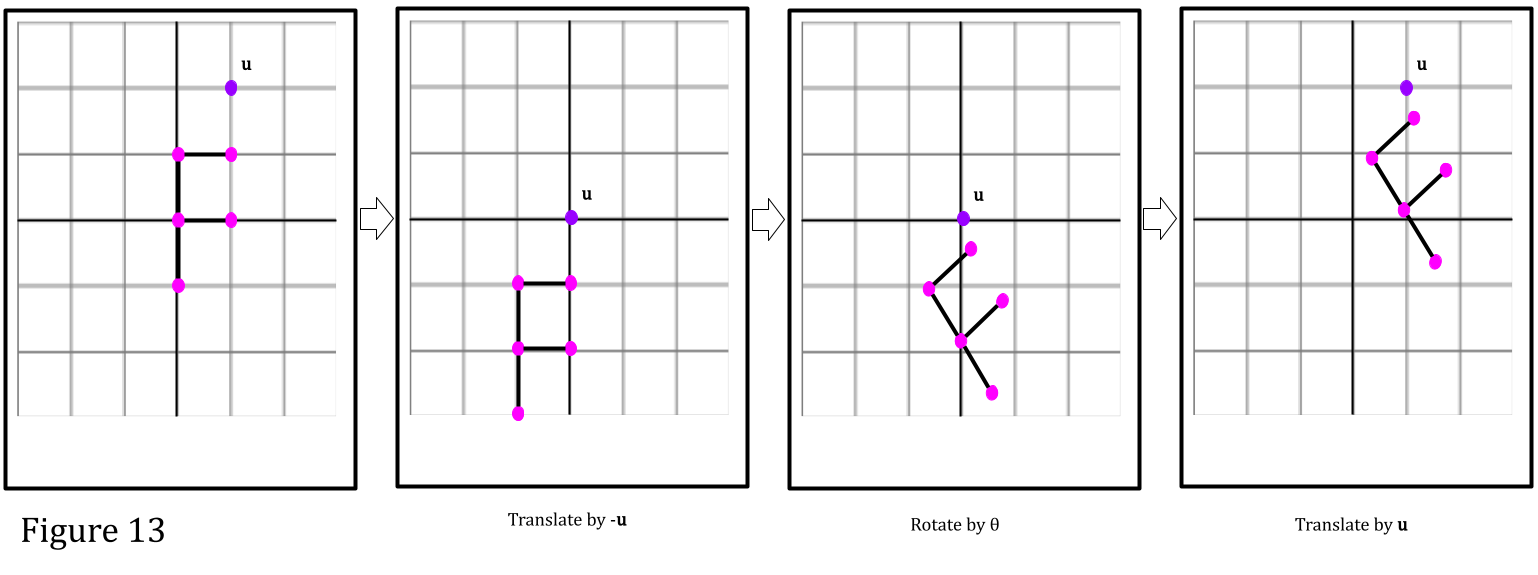
\includegraphics[scale=0.3]{../assets/f12.png}
\end{center}
In general, rotations and translations \textbf{do not commute}. In general, we have 
\[T_{\mathbf{u}} \circ R_{\theta} \neq R_{\theta} \circ T_{\mathbf{u}}.\]

\subsection{Homogeneous Coordinates \& Matrix Representations}
\begin{definition}{}{}
    Let $x, y, w \in \R$ (scalars), assumiwhere $w \neq 0$. Then, the triple 
    \[\cyclic{x, y, w} \text{ or } \begin{bmatrix}
        x \\ y \\ w 
    \end{bmatrix}\]
    is a \textbf{homogenerous} representation of the point 
    \[\cyclic{\frac{x}{w}, \frac{y}{w}} \in \R^2.\]
\end{definition}

\begin{mdframed}[]
    (Example.) Some examples of homogeneous coordinates for $\cyclic{2, 1} \in \R^2$ are: 
    \begin{itemize}
        \item $\cyclic{2, 1, 1}$. 
        \item $\cyclic{4, 2, 2}$. 
        \item $\cyclic{8, 4, 4}$. 
        \item $\cyclic{-2, -1, -1}$. 
    \end{itemize}
\end{mdframed}
How do we give a matrix representation of an affine transformation, over homogeneous coordinates? Let $A(\mathbf{x})$ be affine; in particular,
\[A(\mathbf{x}) = B(\mathbf{x}) + \mathbf{u}.\]
Let $B$ be a linear map, represented by the matrix 
\[\begin{bmatrix}
    a & c \\ b & d
\end{bmatrix}.\]
Let $\mathbf{u} = \begin{bmatrix}
    e \\ f
\end{bmatrix}$. Let $N$ be the $3 \times 3$ matrix 
\[\begin{bmatrix}
    a & c & e \\
    b & d & f \\ 
    0 & 0 & 1
\end{bmatrix}.\]
Let $\begin{bmatrix}
    x \\ y \\ 1
\end{bmatrix}$ be a representation of $\begin{bmatrix}
    x \\ y
\end{bmatrix} \in \R^2$. Then,
\[A\left(\begin{bmatrix}
    x \\ y
\end{bmatrix}\right) = \begin{bmatrix}
    a & c \\ 
    b & d
\end{bmatrix} \begin{bmatrix}
    x \\ y
\end{bmatrix} + \begin{bmatrix}
    e \\ f
\end{bmatrix} = \begin{bmatrix}
    ax + cy + e \\ 
    bx + dy + f
\end{bmatrix}.\]
This gives us the transformation under $A$. Now, we note that 
\[N\left(\begin{bmatrix}
    x \\ y \\ z
\end{bmatrix}\right) = \begin{bmatrix}
    a & c & e \\
    b & d & f \\ 
    0 & 0 & 1
\end{bmatrix} \begin{bmatrix}
    x \\ y \\ 1
\end{bmatrix} = \begin{bmatrix}
    ax + cy + e \\ 
    bx + dy + f \\ 
    1
\end{bmatrix}.\]
This represents a homogeneous representation of the same point as $A(\mathbf{x})$.

\bigskip 

Let us now suppose that $w$ is something other than 1 (the general case). More namely, let us consider $\begin{bmatrix}
    wx \\ wy \\ w
\end{bmatrix}$, where $w \neq 0$. This is another homogeneous representation of the point $\begin{bmatrix}
    x \\ y
\end{bmatrix}$. Then, 
\[N \begin{bmatrix}
    wx \\ wy \\ w
\end{bmatrix} = w N\begin{bmatrix}
    x \\ y \\ 1
\end{bmatrix} = \begin{bmatrix}
    w(ax + cy + e) \\ 
    w(bx + dy + f) \\ 
    w
\end{bmatrix}.\]
This is another homogeneous representation of the point $A\left(\begin{bmatrix}
    x \\ y
\end{bmatrix}\right)$. \emph{Additionally}, for any $\alpha \neq 0$, $\alpha N$ is a $3 \times 3$ matrix that also represents $A(\mathbf{x})$ over homogeneous coordinates. 

\begin{mdframed}[]
    (Example.) Suppose we're given the following affine transformation:
    \begin{center}
        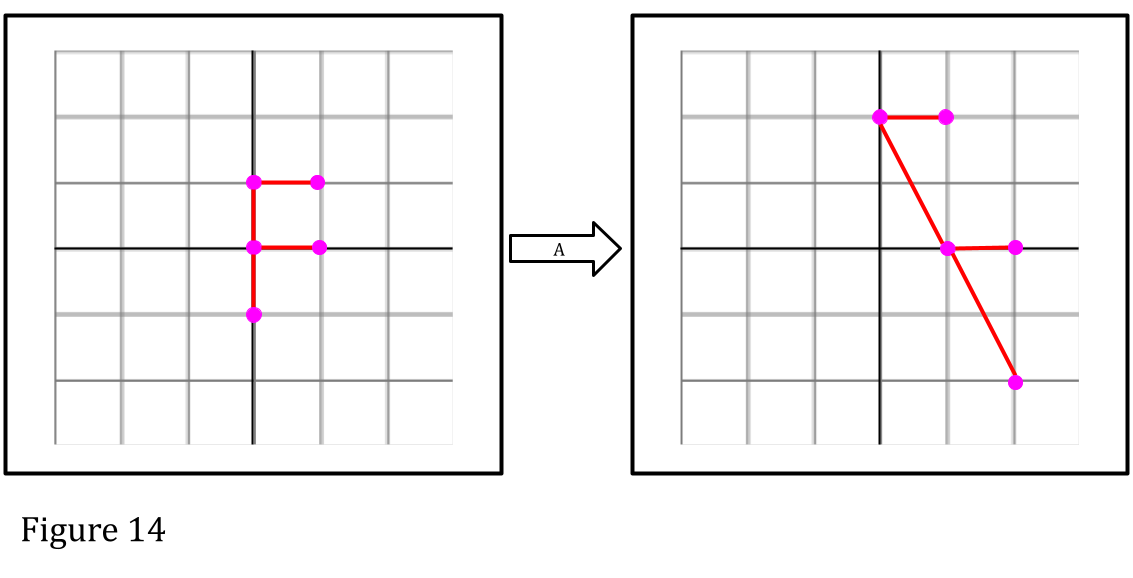
\includegraphics[scale=0.35]{../assets/f13.png}
    \end{center}
    Find a matrix representation of an affine transformation.

    \begin{mdframed}[]
        The matrix representation for $A$ is given by: 
        \[A = \begin{bmatrix}
            1 & -1 & 1 \\ 
            0 & 2 & 0 \\ 
            0 & 0 & 1
        \end{bmatrix}.\]
        In other words, the above matrix is the $3 \times 3$ matrix representation of $A$. To see how we got this answer, we note that the 
        \[\begin{bmatrix}
            A(\mathbf{i}) - \mathbf{i} & A(\mathbf{j}) - \mathbf{j}
        \end{bmatrix} = \begin{bmatrix}
            1 & -1 \\ 
            0 & 2
        \end{bmatrix}\]
        is just the $2 \times 2$ matrix representation of the image, and the 
        \[\begin{bmatrix}
            1 \\ 0
        \end{bmatrix}\]
        is the translation. We keep the bottom 
        \[\begin{bmatrix}
            0 & 0 & 1
        \end{bmatrix}\]
        as is.
    \end{mdframed}
\end{mdframed}

\subsection{Hierarchical Transformations}
Why do we need hierarchical transformations? Suppose we are simulating a moving object which has parts that are moving relative to the objects itself. We want to have some transformations -- representing the movement of the overall object -- and then transformations controlling the cars. So, as an example, if we have a car that is moving, we might have matrices controlling the position of the car; we might also have matrices controlling where, say, the steering wheel or the wheels or the car door are. 

\bigskip 

Consider the following example: 
\begin{center}
    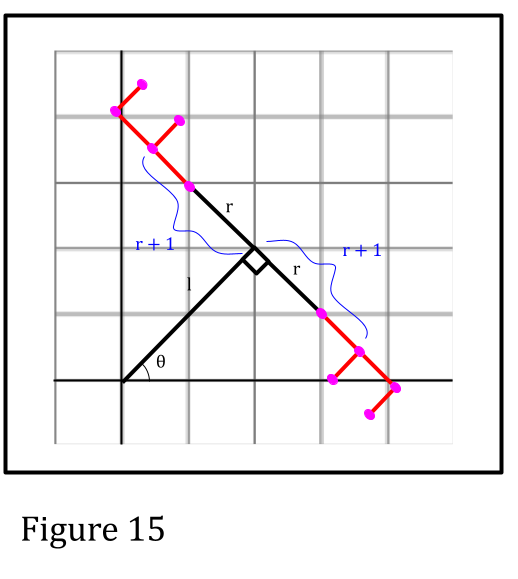
\includegraphics[scale=0.5]{../assets/f14.png}
\end{center}
How do we move a standard ``F''-shape to the upper ``F'' position? If we imagine the right-angle at $(2, 2)$ to be the ``origin,'' then: 
\begin{enumerate}
    \item We can move the standard ``F''-shape upwards $T_{\cyclic{0, r + 1}}$.
    \item Then, we can move the standard ``F''-shape right by $T_{\cyclic{\ell, 0}}$.
    \item Then, we will rotate the ``F''-shape by $\theta$. 
\end{enumerate}
How do we represent this (upper ``F'') in terms of compositions?
\[R_{\theta} \circ T_{\cyclic{\ell, 0}} \circ T_{\cyclic{0, r + 1}}.\]
How about the lower ``F'' position? Again, 
\begin{enumerate}
    \item We rotate the ``F''-shape by $\pi$ (180 degrees).
    \item We then move the ``F''-shape down $T_{\cyclic{0, -(r + 1)}}$. 
    \item We translate the ``F''-shape by $T_{\cyclic{\ell, 0}}$.
    \item Finally, rotate the ``F''-shape by $R_{\theta}$.
\end{enumerate}
This gives us the transformations, in terms of compositions, as 
\[R_{\theta} \circ T_{\ell, 0} \circ T_{\cyclic{0, -(r + 1)}} \circ R_{\pi}.\]

\subsubsection{Application to OpenGL}
How would this (roughly) look in OpenGL?
\begin{verbatim}
    Let T = Theta 
    // Identity matrix 
    M_1 = Identity 
    // Compose with rotation about angle T
    M_1 = M_1 o R_T
    // Compose with translation by (l, 0)
    M_1 = M_1 o T_(l, 0)
    // Compose with translation by (0, r + 1)
    // This gives us the first composition below Figure 15. 
    M_2 = M_1 o T_(0, r + 1)
    Render ''F'' with M_2 as the model view matrix to render upper ''F''

    M_3 = M_1 o T_(0, -(r + 1))
    // This gives us the second composition below Figure 15. 
    M_3 = M_3 o R_pi 
    Render ''F'' with M_3 as the model view matrix. 
\end{verbatim}
In a real OpenGL program,
\begin{itemize}
    \item Transformations are done as matrices acting on homogeneous coordinates. In $\R^3$, we use $4 \times 4$ matrices. 
    \item Compositions is just matrix multiplication. 
    \item Model view matrices get send to shader program as uniform variables. 
    \item The vertex positions are vertex attributes stored in the VBO. 
\end{itemize}

\end{document}